\section{Research Questions}

\begin{question}
Referring to \cref{fig:03-n3-dual}, are there any conserved quantities for the dual family besides stationarity of $X_4$ at the common center?
\end{question}

\begin{question}
Referring to  the dashed green triangle in \cref{fig:03-n3-affine}(middle), are there any conserved quantities and/or fixed triangle centers for the family which is an $s$-affine image of billiard excentrals?
\end{question}

\begin{question}
\textcolor{red}{inversive}
Consider the family of inversive images of excentral triangles with respect to a circle centered at a point $M$ in the plane. Show the symmedian point $X_6$ of such a family will be stationary regardless of $M$. Compute the location of $X_6$. See this curious phenomenon in a \href{https://youtu.be/wwX_QfkjVi0}{Video}.
\end{question}

\begin{question}
Consider the homothetic family and its polar image with respect to a focus of the outer ellipse $\E$. Prove that (i) the caustic is a circle, derive its location and radius. (ii) the family is inscribed in a conic, namely, below (resp. above) a certain aspect ratio $a/b$ of $\E$, the conic is an an ellipse (resp. hyperbola). (iii) the Gergonne point $X_7$ of the family is stationary.
Live: family inscribed in \href{https://bit.ly/33p7xj6}{ellipse}, \href{https://bit.ly/3bbTaTt}{hyperbola}.
\end{question}

\begin{question}
 $X_{57}$ is the isogonal conjugate of $X_9$. Referring to \cref{fig:03-x57}, prove the Brianchon point for the $X_{57}$-centered inconic is $X_{189}$. Prove the 3-periodic family interscribed between the $X_{57}$-centered inconic and circumconic maintains $X_{57}$ stationary. Prove that the normals at the vertices of the $X_{57}$-centered circumconic concur at $X_{3345}$. 
\label{que:03-x57}
\end{question}

\begin{figure}
    \centering
    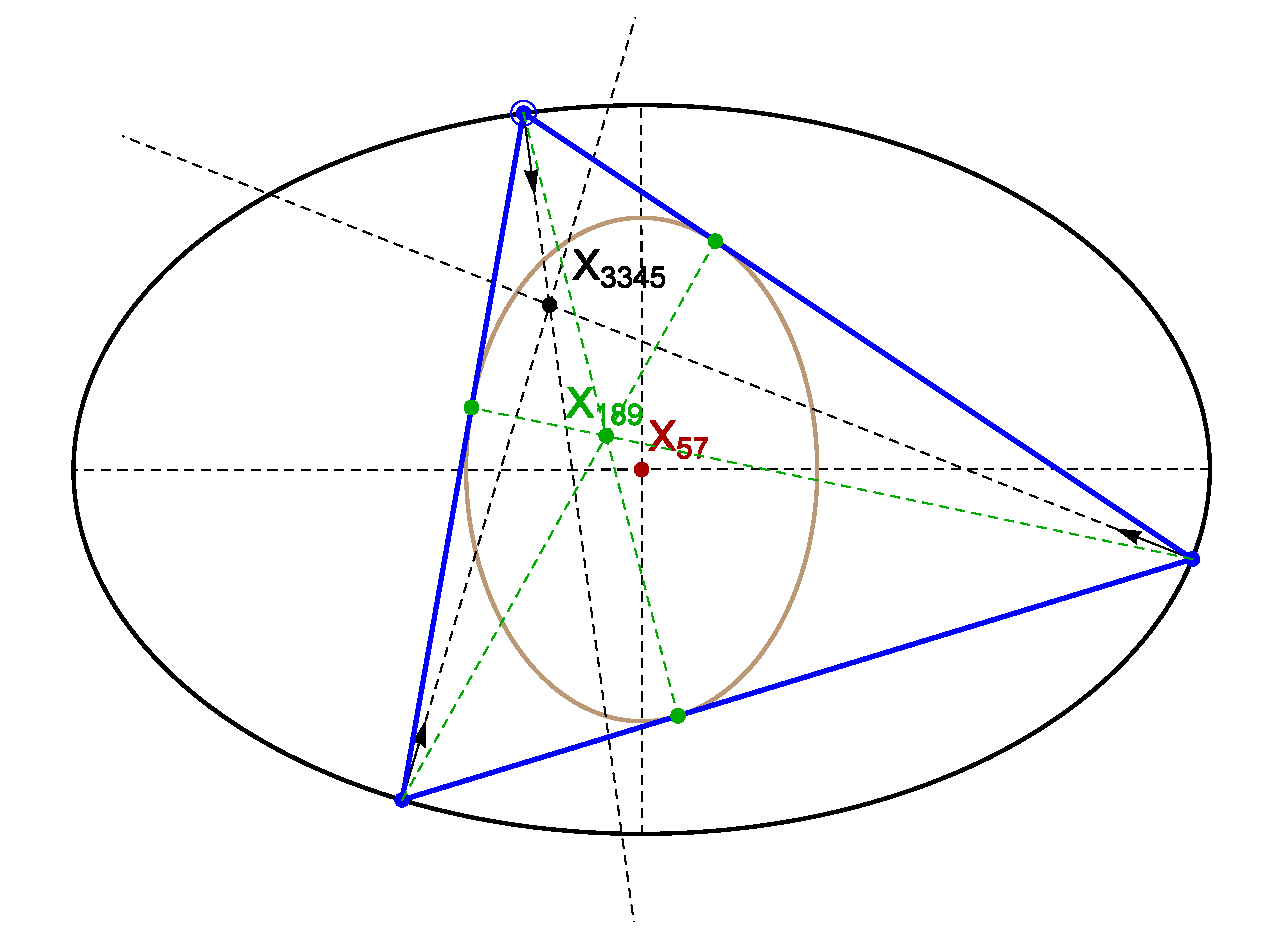
\includegraphics[width=.6\textwidth]{pics_03_310_poncelet_x57.eps}
    \caption{A Poncelet 3-periodic (blue) interscribed between the $X_{57}$-centered circumconic and inconic. $X_{189}$ is the inconic's Brianchon point. Normals at the circumconic vertices concur at $X_{3345}$. $X_{57}$ remains stationary over the family.}
    \label{fig:03-x57}
\end{figure}

\begin{question}
Given a triangle, compute its $X_7$-centered inconic and circumconic. Prove that 3-periodics intersecribed in said conics will not maintain $X_7$ stationary. Prove the same by taking the conic pair's center to be $X_8$ and $X_{10}$, i.e., in neither of these cases will the original center remain stationary. Report the Brianchon point for all said inconics.
\label{que:03-x7}
\end{question}

%\begin{table}
%\centering
%\begin{tabular}{|r|c|c|c|c|c|c|c|}
%\hline
%\makecell[rc]{Poncelet\\family} &
%center &
%\makecell[cc]{norms.\\concur} &
%\makecell[cc]{concur\\ \texttt{bit.ly/*}} & 
%inconic & 
%\makecell[cc]{Brian-\\chon} &
%\makecell[cc]{caustic\\contact tri} &
%\makecell[cc]{contact tri\\ \texttt{bit.ly/*}} \\
%\hline
%incircle & $X_1$ & $X_{84}$ & \href{https://bit.ly/3eVuCQY&}{\texttt{3eVuCQY}} &  %incircle & $X_7$ & intouch & \href{https://bit.ly/3tYYu3h}{\texttt{3tYYu3h}}\\
%homothetic & $X_2$ & $X_4$ & \href{https://bit.ly/3eXSRhC}{\texttt{3eXSRhC}} & %Steiner & $X_2$ & medial & \href{https://bit.ly/3474753}{\texttt{3474753}} \\
%circumcircle & $X_3$ & $X_3$ & \href{https://bit.ly/2RqMqul}{\texttt{2RqMqul}} & ? & %$X_{69}$ & $X_{69}$-cev. & \href{https://bit.ly/2T3qu9f}{\texttt{2T3qu9f}}\\
%dual & $X_4$ & $X_{3346}$ & n/a & ? & $X_{253}$ & $X_{253}$-cev. & %\href{https://bit.ly/2SUfomB}{\texttt{2SUfomB}} \\
%excentral & $X_6$ & $X_{64}$ & \href{https://bit.ly/3hwCTfN}{\texttt{3hwCTfN}} & %orthic & $X_4$ & orthic & \href{https://bit.ly/3uXXI7H}{\texttt{3uXXI7H}}\\
%confocal & $X_9$ & $X_1$ & \href{https://bit.ly/3uTvqLI}{\texttt{3uTvqLI}} & Mandart %& $X_8$ & extouch & \href{https://bit.ly/3wiBeyv}{\texttt{3wiBeyv}} \\
%\hline
%x57 & $X_{57}$ & $X_{3345}$ & n/a & ? & $X_{189}$ &  $X_{189}$-cev. & n/a\\
%\hline
%\end{tabular}
%\caption{Ellipse normal concurrence for various Poncelet families / circumconics.}
%\label{tab:03-normal-concurrence}
%\end{table}

\begin{question}
\label{que:03-thomson}
A triangle cubic is a degree-3 implicit equation on barycentrics with respect to a triangle $T$, see \cite[Triangle cubic]{mw}. The Thomson cubic contains the vertices, sideline midpoints, and the excenters. It is also the locus of points $X$ such that normals at $X$-centered circumconic vertices concur, see \cite{gibert2021-thomson} and \cite[Thomson cubic]{mw}. The first 10 Kimberling centers on this cubic are $X_k$, $k=$1, 2, 3, 4, 6, 9, 57, 223, 282, 1073. The first 6 of these are precisely the centers of the CAP families mentioned herein. Indeed, where their normals concur is shown in \cref{tab:03-normal-concurrence}. Experimentally, the $X_{57}$-centered ellipse pair maintains said point stationary, see \cref{que:03-x57}, while the same is not true for other three centers not on the Thomson cubic, see \cref{que:03-x7}. Prove (or reject) the following conjecture:
\end{question}

\begin{conjecture}
A triangle center $X_k$ is stationary over 3-periodics interscribed between $X_k$-centered inconic and circumconic, iff $X_k$ is on the Thomson cubic.
\end{conjecture}